% Created by tikzDevice version 0.12.6 on 2026-05-16 05:25:08
% !TEX encoding = UTF-8 Unicode
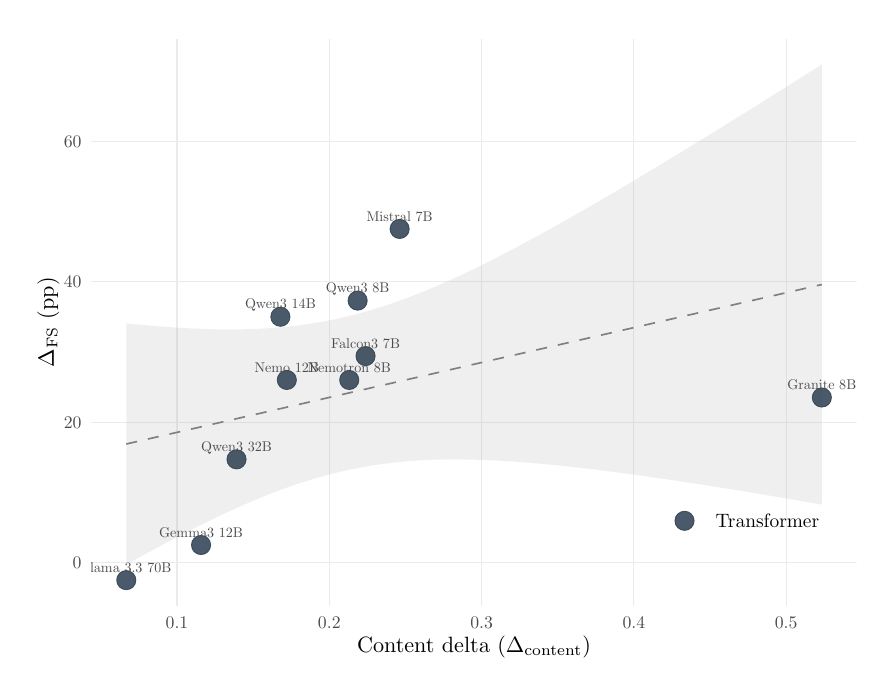
\begin{tikzpicture}[x=1pt,y=1pt]
\definecolor{fillColor}{RGB}{255,255,255}
\path[use as bounding box,fill=fillColor,fill opacity=0.00] (0,0) rectangle (303.53,231.26);
\begin{scope}
\path[clip] (  0.00,  0.00) rectangle (303.53,231.26);
\definecolor{fillColor}{RGB}{255,255,255}

\path[fill=fillColor] (  0.00,  0.00) rectangle (303.53,231.26);
\end{scope}
\begin{scope}
\path[clip] ( 23.06, 22.32) rectangle (299.53,227.26);
\definecolor{drawColor}{gray}{0.92}

\path[draw=drawColor,line width= 0.4pt,line join=round] ( 23.06, 37.98) --
	(299.53, 37.98);

\path[draw=drawColor,line width= 0.4pt,line join=round] ( 23.06, 88.74) --
	(299.53, 88.74);

\path[draw=drawColor,line width= 0.4pt,line join=round] ( 23.06,139.49) --
	(299.53,139.49);

\path[draw=drawColor,line width= 0.4pt,line join=round] ( 23.06,190.25) --
	(299.53,190.25);

\path[draw=drawColor,line width= 0.4pt,line join=round] ( 53.96, 22.32) --
	( 53.96,227.26);

\path[draw=drawColor,line width= 0.4pt,line join=round] (108.99, 22.32) --
	(108.99,227.26);

\path[draw=drawColor,line width= 0.4pt,line join=round] (164.02, 22.32) --
	(164.02,227.26);

\path[draw=drawColor,line width= 0.4pt,line join=round] (219.06, 22.32) --
	(219.06,227.26);

\path[draw=drawColor,line width= 0.4pt,line join=round] (274.09, 22.32) --
	(274.09,227.26);
\definecolor{fillColor}{RGB}{153,153,153}

\path[fill=fillColor,fill opacity=0.15] ( 35.63,124.41) --
	( 38.81,124.09) --
	( 41.99,123.80) --
	( 45.17,123.52) --
	( 48.36,123.26) --
	( 51.54,123.03) --
	( 54.72,122.82) --
	( 57.90,122.64) --
	( 61.08,122.49) --
	( 64.26,122.37) --
	( 67.45,122.28) --
	( 70.63,122.23) --
	( 73.81,122.22) --
	( 76.99,122.25) --
	( 80.17,122.32) --
	( 83.35,122.44) --
	( 86.53,122.62) --
	( 89.72,122.84) --
	( 92.90,123.12) --
	( 96.08,123.46) --
	( 99.26,123.86) --
	(102.44,124.32) --
	(105.62,124.84) --
	(108.80,125.43) --
	(111.99,126.09) --
	(115.17,126.82) --
	(118.35,127.61) --
	(121.53,128.47) --
	(124.71,129.39) --
	(127.89,130.39) --
	(131.07,131.44) --
	(134.26,132.55) --
	(137.44,133.72) --
	(140.62,134.95) --
	(143.80,136.23) --
	(146.98,137.57) --
	(150.16,138.95) --
	(153.34,140.37) --
	(156.53,141.83) --
	(159.71,143.34) --
	(162.89,144.88) --
	(166.07,146.46) --
	(169.25,148.06) --
	(172.43,149.70) --
	(175.62,151.36) --
	(178.80,153.05) --
	(181.98,154.76) --
	(185.16,156.50) --
	(188.34,158.25) --
	(191.52,160.03) --
	(194.70,161.82) --
	(197.89,163.62) --
	(201.07,165.45) --
	(204.25,167.28) --
	(207.43,169.13) --
	(210.61,171.00) --
	(213.79,172.87) --
	(216.97,174.75) --
	(220.16,176.65) --
	(223.34,178.55) --
	(226.52,180.47) --
	(229.70,182.39) --
	(232.88,184.32) --
	(236.06,186.25) --
	(239.24,188.20) --
	(242.43,190.15) --
	(245.61,192.10) --
	(248.79,194.06) --
	(251.97,196.03) --
	(255.15,198.00) --
	(258.33,199.98) --
	(261.52,201.96) --
	(264.70,203.94) --
	(267.88,205.93) --
	(271.06,207.93) --
	(274.24,209.93) --
	(277.42,211.93) --
	(280.60,213.93) --
	(283.79,215.94) --
	(286.97,217.95) --
	(286.97, 58.93) --
	(283.79, 59.49) --
	(280.60, 60.03) --
	(277.42, 60.58) --
	(274.24, 61.12) --
	(271.06, 61.66) --
	(267.88, 62.20) --
	(264.70, 62.73) --
	(261.52, 63.25) --
	(258.33, 63.78) --
	(255.15, 64.29) --
	(251.97, 64.81) --
	(248.79, 65.32) --
	(245.61, 65.82) --
	(242.43, 66.32) --
	(239.24, 66.81) --
	(236.06, 67.29) --
	(232.88, 67.77) --
	(229.70, 68.24) --
	(226.52, 68.70) --
	(223.34, 69.16) --
	(220.16, 69.60) --
	(216.97, 70.04) --
	(213.79, 70.46) --
	(210.61, 70.88) --
	(207.43, 71.28) --
	(204.25, 71.67) --
	(201.07, 72.05) --
	(197.89, 72.42) --
	(194.70, 72.76) --
	(191.52, 73.10) --
	(188.34, 73.41) --
	(185.16, 73.71) --
	(181.98, 73.98) --
	(178.80, 74.24) --
	(175.62, 74.47) --
	(172.43, 74.67) --
	(169.25, 74.85) --
	(166.07, 75.00) --
	(162.89, 75.11) --
	(159.71, 75.20) --
	(156.53, 75.24) --
	(153.34, 75.25) --
	(150.16, 75.21) --
	(146.98, 75.14) --
	(143.80, 75.01) --
	(140.62, 74.83) --
	(137.44, 74.60) --
	(134.26, 74.31) --
	(131.07, 73.97) --
	(127.89, 73.56) --
	(124.71, 73.10) --
	(121.53, 72.56) --
	(118.35, 71.96) --
	(115.17, 71.30) --
	(111.99, 70.57) --
	(108.80, 69.76) --
	(105.62, 68.90) --
	(102.44, 67.96) --
	( 99.26, 66.97) --
	( 96.08, 65.91) --
	( 92.90, 64.79) --
	( 89.72, 63.61) --
	( 86.53, 62.37) --
	( 83.35, 61.08) --
	( 80.17, 59.75) --
	( 76.99, 58.36) --
	( 73.81, 56.93) --
	( 70.63, 55.46) --
	( 67.45, 53.95) --
	( 64.26, 52.41) --
	( 61.08, 50.83) --
	( 57.90, 49.22) --
	( 54.72, 47.58) --
	( 51.54, 45.91) --
	( 48.36, 44.22) --
	( 45.17, 42.51) --
	( 41.99, 40.77) --
	( 38.81, 39.01) --
	( 35.63, 37.24) --
	cycle;

\path[] ( 35.63,124.41) --
	( 38.81,124.09) --
	( 41.99,123.80) --
	( 45.17,123.52) --
	( 48.36,123.26) --
	( 51.54,123.03) --
	( 54.72,122.82) --
	( 57.90,122.64) --
	( 61.08,122.49) --
	( 64.26,122.37) --
	( 67.45,122.28) --
	( 70.63,122.23) --
	( 73.81,122.22) --
	( 76.99,122.25) --
	( 80.17,122.32) --
	( 83.35,122.44) --
	( 86.53,122.62) --
	( 89.72,122.84) --
	( 92.90,123.12) --
	( 96.08,123.46) --
	( 99.26,123.86) --
	(102.44,124.32) --
	(105.62,124.84) --
	(108.80,125.43) --
	(111.99,126.09) --
	(115.17,126.82) --
	(118.35,127.61) --
	(121.53,128.47) --
	(124.71,129.39) --
	(127.89,130.39) --
	(131.07,131.44) --
	(134.26,132.55) --
	(137.44,133.72) --
	(140.62,134.95) --
	(143.80,136.23) --
	(146.98,137.57) --
	(150.16,138.95) --
	(153.34,140.37) --
	(156.53,141.83) --
	(159.71,143.34) --
	(162.89,144.88) --
	(166.07,146.46) --
	(169.25,148.06) --
	(172.43,149.70) --
	(175.62,151.36) --
	(178.80,153.05) --
	(181.98,154.76) --
	(185.16,156.50) --
	(188.34,158.25) --
	(191.52,160.03) --
	(194.70,161.82) --
	(197.89,163.62) --
	(201.07,165.45) --
	(204.25,167.28) --
	(207.43,169.13) --
	(210.61,171.00) --
	(213.79,172.87) --
	(216.97,174.75) --
	(220.16,176.65) --
	(223.34,178.55) --
	(226.52,180.47) --
	(229.70,182.39) --
	(232.88,184.32) --
	(236.06,186.25) --
	(239.24,188.20) --
	(242.43,190.15) --
	(245.61,192.10) --
	(248.79,194.06) --
	(251.97,196.03) --
	(255.15,198.00) --
	(258.33,199.98) --
	(261.52,201.96) --
	(264.70,203.94) --
	(267.88,205.93) --
	(271.06,207.93) --
	(274.24,209.93) --
	(277.42,211.93) --
	(280.60,213.93) --
	(283.79,215.94) --
	(286.97,217.95);

\path[] (286.97, 58.93) --
	(283.79, 59.49) --
	(280.60, 60.03) --
	(277.42, 60.58) --
	(274.24, 61.12) --
	(271.06, 61.66) --
	(267.88, 62.20) --
	(264.70, 62.73) --
	(261.52, 63.25) --
	(258.33, 63.78) --
	(255.15, 64.29) --
	(251.97, 64.81) --
	(248.79, 65.32) --
	(245.61, 65.82) --
	(242.43, 66.32) --
	(239.24, 66.81) --
	(236.06, 67.29) --
	(232.88, 67.77) --
	(229.70, 68.24) --
	(226.52, 68.70) --
	(223.34, 69.16) --
	(220.16, 69.60) --
	(216.97, 70.04) --
	(213.79, 70.46) --
	(210.61, 70.88) --
	(207.43, 71.28) --
	(204.25, 71.67) --
	(201.07, 72.05) --
	(197.89, 72.42) --
	(194.70, 72.76) --
	(191.52, 73.10) --
	(188.34, 73.41) --
	(185.16, 73.71) --
	(181.98, 73.98) --
	(178.80, 74.24) --
	(175.62, 74.47) --
	(172.43, 74.67) --
	(169.25, 74.85) --
	(166.07, 75.00) --
	(162.89, 75.11) --
	(159.71, 75.20) --
	(156.53, 75.24) --
	(153.34, 75.25) --
	(150.16, 75.21) --
	(146.98, 75.14) --
	(143.80, 75.01) --
	(140.62, 74.83) --
	(137.44, 74.60) --
	(134.26, 74.31) --
	(131.07, 73.97) --
	(127.89, 73.56) --
	(124.71, 73.10) --
	(121.53, 72.56) --
	(118.35, 71.96) --
	(115.17, 71.30) --
	(111.99, 70.57) --
	(108.80, 69.76) --
	(105.62, 68.90) --
	(102.44, 67.96) --
	( 99.26, 66.97) --
	( 96.08, 65.91) --
	( 92.90, 64.79) --
	( 89.72, 63.61) --
	( 86.53, 62.37) --
	( 83.35, 61.08) --
	( 80.17, 59.75) --
	( 76.99, 58.36) --
	( 73.81, 56.93) --
	( 70.63, 55.46) --
	( 67.45, 53.95) --
	( 64.26, 52.41) --
	( 61.08, 50.83) --
	( 57.90, 49.22) --
	( 54.72, 47.58) --
	( 51.54, 45.91) --
	( 48.36, 44.22) --
	( 45.17, 42.51) --
	( 41.99, 40.77) --
	( 38.81, 39.01) --
	( 35.63, 37.24);
\definecolor{drawColor}{gray}{0.50}

\path[draw=drawColor,line width= 0.6pt,dash pattern=on 4pt off 4pt ,line join=round] ( 35.63, 80.82) --
	( 38.81, 81.55) --
	( 41.99, 82.28) --
	( 45.17, 83.01) --
	( 48.36, 83.74) --
	( 51.54, 84.47) --
	( 54.72, 85.20) --
	( 57.90, 85.93) --
	( 61.08, 86.66) --
	( 64.26, 87.39) --
	( 67.45, 88.12) --
	( 70.63, 88.85) --
	( 73.81, 89.58) --
	( 76.99, 90.31) --
	( 80.17, 91.04) --
	( 83.35, 91.76) --
	( 86.53, 92.49) --
	( 89.72, 93.22) --
	( 92.90, 93.95) --
	( 96.08, 94.68) --
	( 99.26, 95.41) --
	(102.44, 96.14) --
	(105.62, 96.87) --
	(108.80, 97.60) --
	(111.99, 98.33) --
	(115.17, 99.06) --
	(118.35, 99.79) --
	(121.53,100.52) --
	(124.71,101.25) --
	(127.89,101.97) --
	(131.07,102.70) --
	(134.26,103.43) --
	(137.44,104.16) --
	(140.62,104.89) --
	(143.80,105.62) --
	(146.98,106.35) --
	(150.16,107.08) --
	(153.34,107.81) --
	(156.53,108.54) --
	(159.71,109.27) --
	(162.89,110.00) --
	(166.07,110.73) --
	(169.25,111.46) --
	(172.43,112.19) --
	(175.62,112.91) --
	(178.80,113.64) --
	(181.98,114.37) --
	(185.16,115.10) --
	(188.34,115.83) --
	(191.52,116.56) --
	(194.70,117.29) --
	(197.89,118.02) --
	(201.07,118.75) --
	(204.25,119.48) --
	(207.43,120.21) --
	(210.61,120.94) --
	(213.79,121.67) --
	(216.97,122.40) --
	(220.16,123.13) --
	(223.34,123.85) --
	(226.52,124.58) --
	(229.70,125.31) --
	(232.88,126.04) --
	(236.06,126.77) --
	(239.24,127.50) --
	(242.43,128.23) --
	(245.61,128.96) --
	(248.79,129.69) --
	(251.97,130.42) --
	(255.15,131.15) --
	(258.33,131.88) --
	(261.52,132.61) --
	(264.70,133.34) --
	(267.88,134.06) --
	(271.06,134.79) --
	(274.24,135.52) --
	(277.42,136.25) --
	(280.60,136.98) --
	(283.79,137.71) --
	(286.97,138.44);
\definecolor{drawColor}{RGB}{44,62,80}
\definecolor{fillColor}{RGB}{44,62,80}

\path[draw=drawColor,draw opacity=0.85,line width= 0.3pt,line join=round,line cap=round,fill=fillColor,fill opacity=0.85] (122.09,112.59) circle (  3.47);

\path[draw=drawColor,draw opacity=0.85,line width= 0.3pt,line join=round,line cap=round,fill=fillColor,fill opacity=0.85] ( 62.65, 44.32) circle (  3.47);

\path[draw=drawColor,draw opacity=0.85,line width= 0.3pt,line join=round,line cap=round,fill=fillColor,fill opacity=0.85] (286.97, 97.62) circle (  3.47);

\path[draw=drawColor,draw opacity=0.85,line width= 0.3pt,line join=round,line cap=round,fill=fillColor,fill opacity=0.85] ( 35.63, 31.63) circle (  3.47);

\path[draw=drawColor,draw opacity=0.85,line width= 0.3pt,line join=round,line cap=round,fill=fillColor,fill opacity=0.85] (134.41,158.53) circle (  3.47);

\path[draw=drawColor,draw opacity=0.85,line width= 0.3pt,line join=round,line cap=round,fill=fillColor,fill opacity=0.85] ( 93.64,103.96) circle (  3.47);

\path[draw=drawColor,draw opacity=0.85,line width= 0.3pt,line join=round,line cap=round,fill=fillColor,fill opacity=0.85] (116.20,103.96) circle (  3.47);

\path[draw=drawColor,draw opacity=0.85,line width= 0.3pt,line join=round,line cap=round,fill=fillColor,fill opacity=0.85] ( 91.32,126.80) circle (  3.47);

\path[draw=drawColor,draw opacity=0.85,line width= 0.3pt,line join=round,line cap=round,fill=fillColor,fill opacity=0.85] ( 75.47, 75.28) circle (  3.47);

\path[draw=drawColor,draw opacity=0.85,line width= 0.3pt,line join=round,line cap=round,fill=fillColor,fill opacity=0.85] (119.23,132.64) circle (  3.47);
\definecolor{drawColor}{gray}{0.30}

\node[text=drawColor,anchor=base,inner sep=0pt, outer sep=0pt, scale=  0.51] at (122.09,115.41) {Falcon3 7B};

\node[text=drawColor,anchor=base,inner sep=0pt, outer sep=0pt, scale=  0.51] at ( 62.65, 47.14) {Gemma3 12B};

\node[text=drawColor,anchor=base,inner sep=0pt, outer sep=0pt, scale=  0.51] at (286.97,100.44) {Granite 8B};

\node[text=drawColor,anchor=base,inner sep=0pt, outer sep=0pt, scale=  0.51] at ( 35.63, 34.45) {Llama 3.3 70B};

\node[text=drawColor,anchor=base,inner sep=0pt, outer sep=0pt, scale=  0.51] at (134.41,161.35) {Mistral 7B};

\node[text=drawColor,anchor=base,inner sep=0pt, outer sep=0pt, scale=  0.51] at ( 93.64,106.78) {Nemo 12B};

\node[text=drawColor,anchor=base,inner sep=0pt, outer sep=0pt, scale=  0.51] at (116.20,106.78) {Nemotron 8B};

\node[text=drawColor,anchor=base,inner sep=0pt, outer sep=0pt, scale=  0.51] at ( 91.32,129.63) {Qwen3 14B};

\node[text=drawColor,anchor=base,inner sep=0pt, outer sep=0pt, scale=  0.51] at ( 75.47, 78.11) {Qwen3 32B};

\node[text=drawColor,anchor=base,inner sep=0pt, outer sep=0pt, scale=  0.51] at (119.23,135.46) {Qwen3 8B};
\end{scope}
\begin{scope}
\path[clip] (  0.00,  0.00) rectangle (303.53,231.26);
\definecolor{drawColor}{gray}{0.30}

\node[text=drawColor,anchor=base east,inner sep=0pt, outer sep=0pt, scale=  0.64] at ( 19.46, 35.77) {0};

\node[text=drawColor,anchor=base east,inner sep=0pt, outer sep=0pt, scale=  0.64] at ( 19.46, 86.53) {20};

\node[text=drawColor,anchor=base east,inner sep=0pt, outer sep=0pt, scale=  0.64] at ( 19.46,137.29) {40};

\node[text=drawColor,anchor=base east,inner sep=0pt, outer sep=0pt, scale=  0.64] at ( 19.46,188.05) {60};
\end{scope}
\begin{scope}
\path[clip] (  0.00,  0.00) rectangle (303.53,231.26);
\definecolor{drawColor}{gray}{0.30}

\node[text=drawColor,anchor=base,inner sep=0pt, outer sep=0pt, scale=  0.64] at ( 53.96, 14.31) {0.1};

\node[text=drawColor,anchor=base,inner sep=0pt, outer sep=0pt, scale=  0.64] at (108.99, 14.31) {0.2};

\node[text=drawColor,anchor=base,inner sep=0pt, outer sep=0pt, scale=  0.64] at (164.02, 14.31) {0.3};

\node[text=drawColor,anchor=base,inner sep=0pt, outer sep=0pt, scale=  0.64] at (219.06, 14.31) {0.4};

\node[text=drawColor,anchor=base,inner sep=0pt, outer sep=0pt, scale=  0.64] at (274.09, 14.31) {0.5};
\end{scope}
\begin{scope}
\path[clip] (  0.00,  0.00) rectangle (303.53,231.26);
\definecolor{drawColor}{RGB}{0,0,0}

\node[text=drawColor,anchor=base,inner sep=0pt, outer sep=0pt, scale=  0.80] at (161.30,  5.56) {Content delta ($\Delta_{\mathrm{content}}$)};
\end{scope}
\begin{scope}
\path[clip] (  0.00,  0.00) rectangle (303.53,231.26);
\definecolor{drawColor}{RGB}{0,0,0}

\node[text=drawColor,rotate= 90.00,anchor=base,inner sep=0pt, outer sep=0pt, scale=  0.80] at (  9.51,124.79) {$\Delta_{\mathrm{FS}}$ (pp)};
\end{scope}
\begin{scope}
\path[clip] (  0.00,  0.00) rectangle (303.53,231.26);
\definecolor{drawColor}{RGB}{44,62,80}
\definecolor{fillColor}{RGB}{44,62,80}

\path[draw=drawColor,draw opacity=0.85,line width= 0.3pt,line join=round,line cap=round,fill=fillColor,fill opacity=0.85] (237.35, 53.06) circle (  3.47);
\end{scope}
\begin{scope}
\path[clip] (  0.00,  0.00) rectangle (303.53,231.26);
\definecolor{drawColor}{RGB}{0,0,0}

\node[text=drawColor,anchor=base west,inner sep=0pt, outer sep=0pt, scale=  0.70] at (248.58, 50.65) {Transformer};
\end{scope}
\end{tikzpicture}
